\documentclass[fleqn]{article}
\usepackage{amsmath}
\usepackage{amsfonts} 
\usepackage{graphicx}
\usepackage{tabularx}
\usepackage{listings}

\begin{document}
\newcommand\tab[1][1cm]{\hspace*{#1}}
\section*{Numerical Optimization with Python -  Ex. 2: dry part}
Alon\\ \\

The code I used to create the drawings can be found at:\\

\begin{lstlisting}[breaklines]
https://github.com/Amannor/python_numerical_optimizations/tree/main/ex2/dry_part
\end{lstlisting}

\underline{\textbf{Question 1}}:\\

\underline{\textbf{1.1}} \\
See figure below. \\

\begin{figure}[h!]
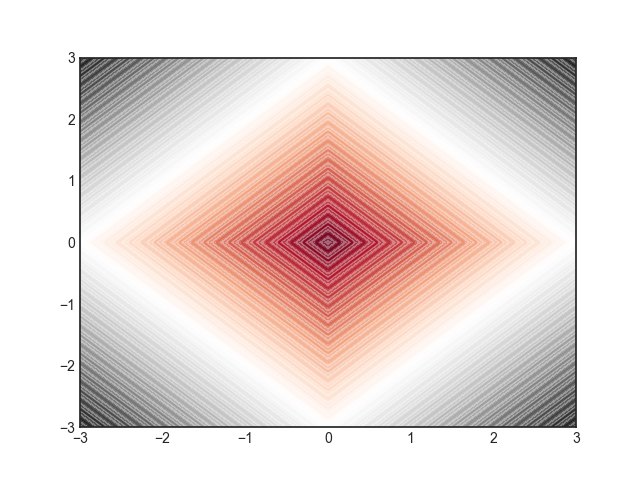
\includegraphics[width=0.8\linewidth]{q1_1.PNG}
\caption{Q1.1: contour lines of $\lvert x\rvert +\lvert y \rvert$}
\end{figure}

\underline{\textbf{1.2}} \\
I wasn't able to draw everything in a single figure, so see 2 figure below:\\
- The feasible region on top of the contour of the objective function. \\
- The contours of the constraints (without the objective function). \\

The constraint $(x-1)^2+(y-1)^2 \leq 1$ yields a circle of radius 1 with a center in (1,1). Adding to it the constraint $y \leq 1$ makes the said circle a (lower) half circle.\\

*I used the following link to find the minimum value: \\
\begin{lstlisting}[breaklines]
https://www.wolframalpha.com/input/?i=min+%7Cx%7C+%2B%7Cy%7C%2C+%28x-1%29%5E2+%2B+%28y-1%29%5E2%3C%3D1%2C+y%3C%3D1
\end{lstlisting} 

\begin{figure}[h!]
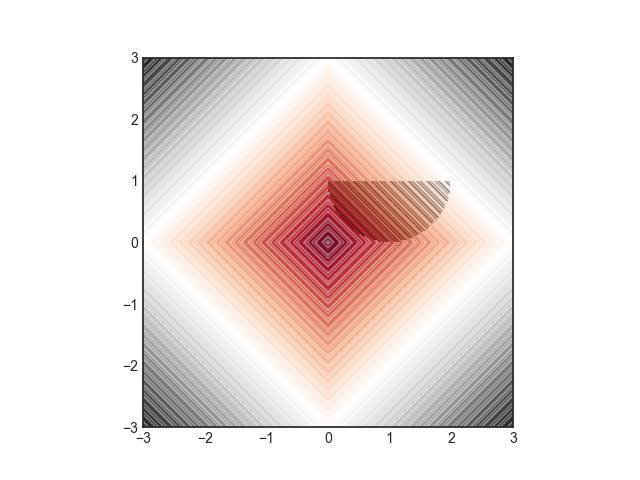
\includegraphics[width=0.8\linewidth]{q1_2.PNG}
\caption{Q1.2: Contour lines of the objective function $f_0(x,y) = \lvert x\rvert +\lvert y \rvert$ and the the constraints (feasible region is the black half circle)}
\end{figure}


\begin{figure}[h!]
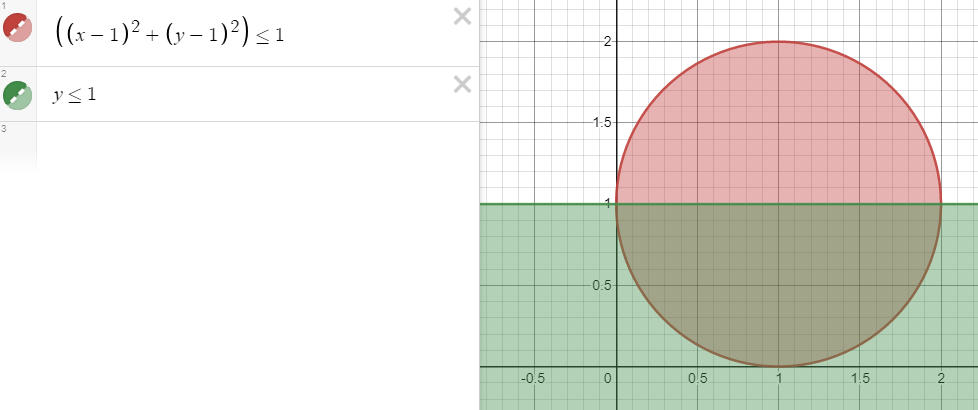
\includegraphics[width=0.8\linewidth]{q1_2_constraints_contours.PNG}
\caption{Q1.2: Contour lines of the constraints functions}
\end{figure}

\underline{\textbf{1.3}} \\
See figure below. \\

Since the minimum of the function  $\lvert x\rvert +\lvert y \rvert $ is at the origin (0,0) and it's monotonically increasing as the (absolute) values of x and y grow, then the minimum in the feasible region is achieved in the closest point to the origin. This point is $(1-\frac{1}{\sqrt{2}}, 1-\frac{1}{\sqrt{2}})$ and is marked in the figure below.\\

The value of the function at this point is $\lvert 1-\frac{1}{\sqrt{2}} \rvert + \lvert1-\frac{1}{\sqrt{2}}\rvert = 2 - \sqrt{2}$\\

\begin{figure}[h!]
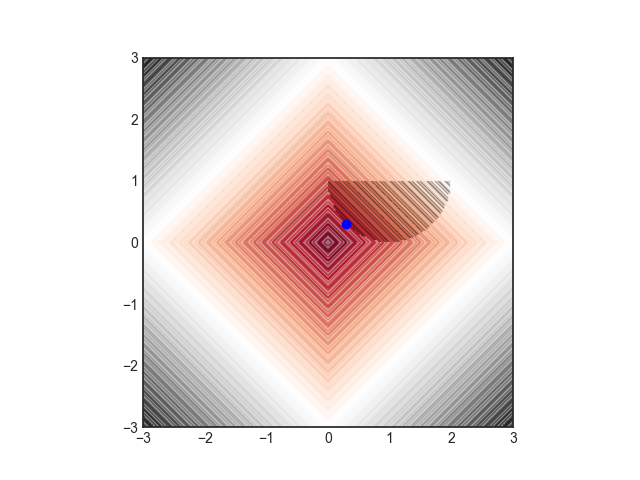
\includegraphics[width=0.8\linewidth]{q1_3.PNG}
\caption{Q1.3: The minimum point in the feasible region is marked in blue}
\end{figure}

\underline{\textbf{1.4}} \\
The constraints are: \\
$f_1 (x,y) = (x-1)^2+(y-1)^2-1 \leq 0$ \\
$f_2 (x,y) = y-1 \leq 0$ \\

We recall that by definition, at a feasible point (x,y), an inequality constraint $ i \in \mathcal{I}$ is said to be active if $f_i (x,y) = 0$ and inactive if $f_i (x,y) < 0$ (lecture 4, slide 7).\\
Hence we'll just assign the value of the minimum point we got above: \\
\begin{multline*}
f_1(1-\frac{1}{\sqrt{2}}, 1-\frac{1}{\sqrt{2}}) = 
(1-\frac{1}{\sqrt{2}}-1)^2 + (1-\frac{1}{\sqrt{2}}-1)^2 -1 = 
\frac{1}{2}+\frac{1}{2}-1 = 0 \\
\rightarrow \boxed{f_1 \; is \; active}
\end{multline*} \\

\begin{multline*}
f_2(1-\frac{1}{\sqrt{2}}, 1-\frac{1}{\sqrt{2}}) = 
1-\frac{1}{\sqrt{2}}-1 = -\frac{1}{\sqrt{2}} < 0 \\
\rightarrow \boxed{f_2 \; is \; not\; active}
\end{multline*} \\

\underline{\textbf{1.5}} \\
See figure below. \\

\begin{figure}[h!]
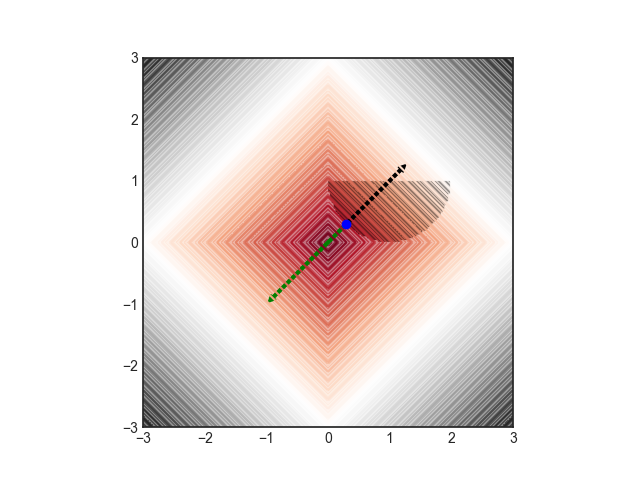
\includegraphics[width=0.8\linewidth]{q1_5.PNG}
\caption{Q1.5: Gradients at minimum point: black is of the objective function and green is of the first constraint $f_1 = (x-1)^2+(y-1)^2-1 \leq 0$}
\end{figure}




\clearpage\underline{\textbf{Question 2}}:\\

\underline{\textbf{2.1}} \\
The graph of the function $f_0(x,y) = 0.5x-y$ is a plane.

I wasn't able to draw everything in a single figure, so see 2 figure below:\\
- The feasible region on top of the contour of the objective function. \\
- The contours of the constraints (without the objective function). \\

Note that for some reason the bottom line of the polygon of the feasible region didn't come out parallel to the x axis as it was suppose to. I'm not sure as to why is that. I went over my code several times and I think it might be related to overflow of values that can't be exactly stored in binary form (e.g. $\frac{1}{3}$).\\

\begin{figure}[h!]
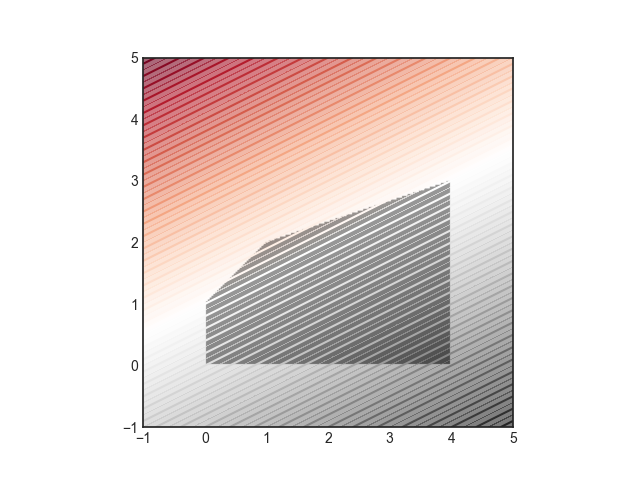
\includegraphics[width=0.8\linewidth]{q2_1.PNG}
\caption{Q2.1: Contours lines of the objective function $0.5x-y$ and the feasible region (in black) given by the constraints}
\end{figure}

\begin{figure}[h!]
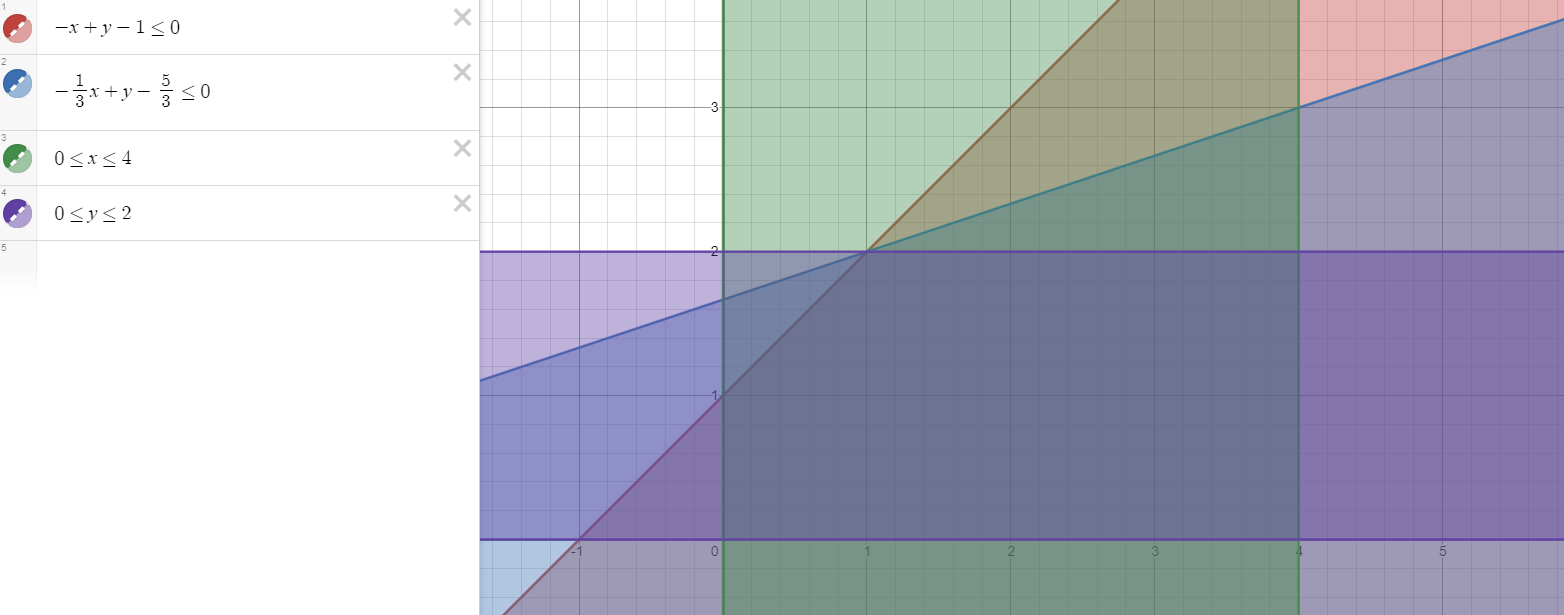
\includegraphics[width=0.8\linewidth]{q2_1_constraints_contours.PNG}
\caption{Q2.1: Contours lines of the constraints functions}
\end{figure}


\underline{\textbf{2.2}} \\
The minimum value is $x^* = (1,2)$ and the optimal value is $p^* = f_0(1,2) = 0.5 \cdot 1 -2 = -1.5$. \\
See figure below.\\

*I used the following link to find the minimum value: \\
\begin{lstlisting}[breaklines]
https://www.wolframalpha.com/input/?i=min+0.5x-y%2C+-x%2By-1%3C%3D0%2C+-x%2F3%2By-5%2F3%3C%3D0%2C+x-4%3C%3D0%2C+y-3%3C%3D0%2C+x%3E%3D0%2C+y%3E%3D0
\end{lstlisting} 

\begin{figure}[h!]
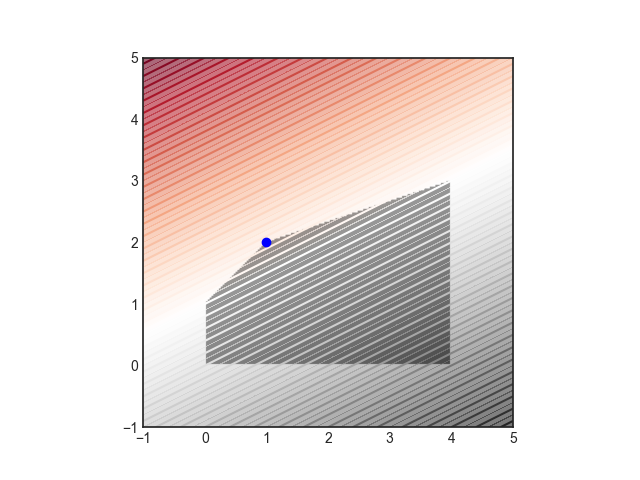
\includegraphics[width=0.8\linewidth]{q2_2.PNG}
\caption{Q2.2: minimum point (1,2) in feasible region is marked in blue}
\end{figure}

\underline{\textbf{2.3}} \\
We'll go over each constraint function and calculate.\\
Of course I wrote (arranged the variables in) each function s.t. the constraint will be $f_i \leq 0 \; (i=1,...,6)$\\

\begin{multline*}
\underline{f_1(x,y) = -x+y-1} \\
f_1(1,2) = -1+2-1 = 0 \rightarrow \boxed{f_1 \; is \; active}
\end{multline*} \\

\begin{multline*}
\underline{f_2(x,y) = -\frac{1}{3}x+y-\frac{5}{3}} \\
f_2(1,2) = -\frac{1}{3}+2-\frac{5}{3} = 0 \rightarrow \boxed{f_2 \; is \; active}
\end{multline*} \\

\begin{multline*}
\underline{f_3(x,y) = x-4} \\
f_3(1,2) = 1-4<0 \rightarrow \boxed{f_3 \; is \; not \; active}
\end{multline*} \\

\begin{multline*}
\underline{f_4(x,y) = y-3} \\
f_4(1,2) = 2-3<0 \rightarrow \boxed{f_4 \; is \; not \; active}
\end{multline*} \\

\begin{multline*}
\underline{f_5(x,y) = -x} \\
f_5(1,2) = -1<0 \rightarrow \boxed{f_5 \; is \; not \; active}
\end{multline*} \\

\begin{multline*}
\underline{f_6(x,y) = -y} \\
f_6(1,2) = -2<0 \rightarrow \boxed{f_6 \; is \; not \; active}
\end{multline*} \\

\underline{\textbf{2.4}} \\
The 2 active constraints are $f_1, f_2$. I've used the following link to "slide" the value of $u$:
\begin{lstlisting}[breaklines]
https://www.desmos.com/calculator/yf5btxc5bz
\end{lstlisting} 

Using it we see that as $u$ decreases in value, the "next" constraint to become active (while $f_1$ becomes inactive) is $f_5$. Hence we can calculate $u_{min}$: \\

$f_5(x,y)=0 \rightarrow -x=0 \rightarrow x=0$\\

$f_1(x,y)=0 \rightarrow -x+y-1=0 \rightarrow y=1$\\

$f_2(x,y)=u_{min} \rightarrow -\frac{1}{3}x+y-\frac{5}{3}=u_{min} =
-\frac{2}{3}$\\


Similarly, as $u$ increases in value, the constraint $f_4$ becomes active

$f_4(x,y)=0 \rightarrow y-3=0 \rightarrow y=3$\\

$f_1(x,y)=0 \rightarrow -x+y-1=0 \rightarrow x=2$\\

$f_2(x,y)=u_{max} \rightarrow -\frac{1}{3}x+y-\frac{5}{3}=u_{max} =
-\frac{2}{3}+3-\frac{5}{3} = \frac{2}{3}$\\


$u_{min} = -\frac{2}{3}, \; u_{max} = \frac{2}{3}$\\


\underline{\textbf{2.5}} \\
we can calculate $x^*(u_{min}), x^*(u_{max})$ (for example by using the wolfram alpha link aforementioned and tweaking constraint $f_2$).\\
We get: \\
$x^*(u_{min}) = (0,1), x^*(u_{max}) = (2,3)$. In between we get that the minimum point "slides" on the graph of $f_1$, hence: \\

$x^*(u) = (x,x+1) \; (u \in [u_{min}, u_{max}], x \in [0,2])$\\

And the optimal value $p^*(u)$ is simply the value of the objective function ($f_0(x,y) = 0.5x-y$) at $x^*(u)$: \\

$p^*(u) = f_0(x^*(u)) \; (u \in [u_{min}, u_{max}], x \in [0,2])$\\

Of course that's not enough since we need to express $x^*(u), p^*(u)$ in terms of $u$. For that we'll remember that for $u \in [u_{min}, u_{max}]$, the active constraints are $f_1, f_2$ so we get:\\

$-x + y - 1 = 0 \rightarrow y=x+1$\\
$-\frac{1}{3}x + y - \frac{5}{3} - u = 0 \rightarrow
-\frac{1}{3}x + x + 1 - \frac{5}{3} - u = 0 \rightarrow
\frac{2}{3}x = u+\frac{2}{3} \rightarrow \\
x = \frac{3}{2}u+1, y = \frac{3}{2}u+2, \; 
\boxed{x^*(u) = \begin{pmatrix}
           \frac{3}{2}u+1 \\
           \frac{3}{2}u+2 
         \end{pmatrix}}$\\
        

$\boxed{p^*(u) = \frac{1}{2} \left( \frac{3}{2}u+1 \right) - \frac{3}{2}u-2 = 
-\frac{3}{4}u-\frac{3}{2}}$\\

$u \in [-\frac{2}{3}, \frac{2}{3}]$ \\


\underline{\textbf{2.6}} \\
$p^*(u)$ is differentiable at u=0. The derivative is:\\
$\frac{\partial p^*(u)}{\partial u} (0) = -\frac{3}{4}$\\
According to definition of optimal dual variable (lecture 6, slide 48): \\
$\lambda ^* = -\frac{\partial p^*(u)}{\partial u}(0) = \frac{3}{4}$


\underline{\textbf{2.7}} \\
See 2 figures below. \\

\begin{figure}[h!]
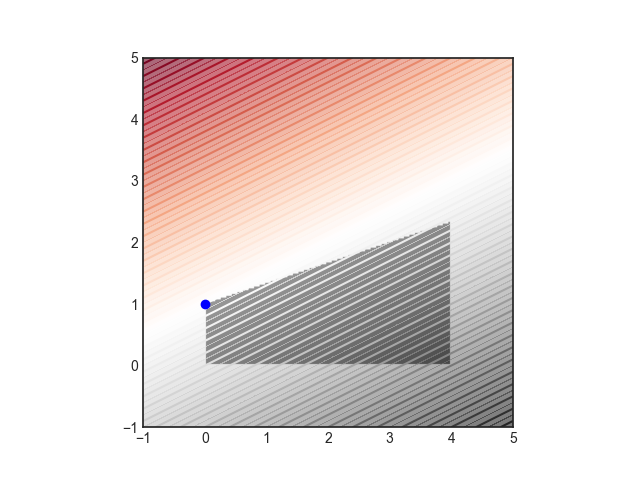
\includegraphics[width=0.8\linewidth]{q2_7_u_min.PNG}
\caption{Q2.7 for $u_{min}=-\frac{2}{3}$: minimum point (0,1) is marked in blue}
\end{figure}

\begin{figure}[h!]
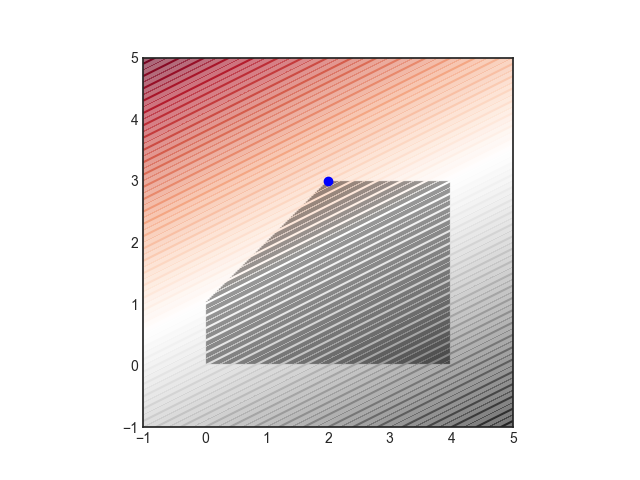
\includegraphics[width=0.8\linewidth]{q2_7_u_max.PNG}
\caption{Q2.7 for $u_{max}=\frac{2}{3}$: minimum point (2,3) is marked in blue}
\end{figure}

\underline{\textbf{2.8}} \\

We'll divide into sections: \\

\underline{$u<-3$} \\

This case is the simplest since it doesn't have any minimum. One can easily see in the following link the area of the intersection of all the constraints becomes an empty set exactly where $u$ passes the threshold of the value of 3: \\
\begin{lstlisting}[breaklines]
https://www.desmos.com/calculator/iclrgw00jl
\end{lstlisting}


\underline{$u=-3$} \\
$x^*(u) = (4,0), \; p^*(u) = 0.5 \cdot 4 -0 = 2$ \\

\begin{multline*}
f_1(4,0) = -4+0-1 < 0 \rightarrow \boxed{f_1 \; is \; not \; active} \\
f_2(4,0) = -\frac{4}{3}+0-\frac{5}{3}+3 = 0 \rightarrow \boxed{f_2 \; is  \; active} \\
f_3(4,0) = 4-4=0 \rightarrow \boxed{f_3 \; is  \; active} \\
f_4(4,0) = 0-3<0 \rightarrow \boxed{f_4 \; is \; not \; active} \\
f_5(4,0) = -4<0 \rightarrow \boxed{f_5 \; is \; not \; active} \\
f_6(4,0) = 0=0 \rightarrow \boxed{f_6 \; is \; active} \\
\end{multline*} \\




Source:
\begin{lstlisting}[breaklines]
https://www.wolframalpha.com/input/?i=min+0.5x-y%2C+-x%2By-1%3C%3D0%2C+-x%2F3%2By-5%2F3%3C%3D-3%2C+x-4%3C%3D0%2C+y-3%3C%3D0%2C+x%3E%3D0%2C+y%3E%3D0
\end{lstlisting}


\underline{$-3<u<u_i$} \\

Working our way "up" (i.e. increasing the value of u, s.t. $u>-3$) we see that the the constraint $f_6$ is active. As we get to the next intersection point, the next constraint to be active is $f_5$. Let's denote the value of u in that point as $u_i$, and calculate it: \\
$f_5 \; active \rightarrow x=0, \;\; f_6 \; active \rightarrow y=0, \;\; f_2 \; active \rightarrow \boxed{u_i = -\frac{1}{3} \cdot 0 + 0 -\frac{5}{3} = -\frac{5}{3}}$ \\
In the interval $u \in [-\frac{5}{3},-3]$ we get (from $f_6(x,y)=0$) that y=0  and (from $f_2(x,y)=0$) x is:
$x = -3 \cdot(u+\frac{5}{3}) = -3u-5$\\

So we can summarize the interval of u until now:\\

\underline{$-3 \leq u \leq -\frac{5}{3}$} \\
$\boxed{x^*(u) = \begin{pmatrix}
           -3u-5 \\
           0 
         \end{pmatrix}}$
$\boxed{p^*(u) = -\frac{3u+5}{2}}$ \\

\underline{$-\frac{5}{3} \leq u \leq -\frac{2}{3}$} \\
Since $f_5$ is active we get x=0. From $f_2$ being active we get: $y = u+\frac{1}{3}\cdot 0 +\frac{5}{3} = u +\frac{5}{3}$.\\
So we get: \\

$\boxed{x^*(u) = \begin{pmatrix}
           0 \\
           u +\frac{5}{3} 
         \end{pmatrix}}$
$\boxed{p^*(u) = -u -\frac{5}{3}}$ \\

\underline{\textbf{2.9}} \\

\underline{$u \geq u_{max} (=\frac{2}{3})$} \\

Here again we'll call upon the help of the desmos link (aforementioned) to help us get a geometrical intuition as to what happens in this case. It's clear that the intersection area between all the functions of the constrains doesn't change for values of u that exceed $u_{max}$. Hence for all $u \geq u_{max}$, the values of $x^*(u), p^*(u)$ are the same as when $u=\frac{2}{3}$ and can be calculated from what we calculated in 2.5 above:\\
$x^*(u) = (\frac{3}{2}u+1, \frac{3}{2}u+2) = (\frac{3}{2} \cdot \frac{2}{3}+1, \frac{3}{2}\cdot \frac{2}{3}+2) = (2,3)$ \\

$p^*(u) = -\frac{3}{4}u-\frac{3}{2} = -\frac{3}{4}\cdot \frac{2}{3}-\frac{3}{2} = -2$

As for the constraints: \\

\begin{multline*}
f_1(2,3) = -2+3-1 = 0 \rightarrow \boxed{f_1 \; is \; active} \\
f_2(2,3) = -\frac{2}{3}+3-\frac{5}{3}-\frac{2}{3} = 0 \rightarrow \boxed{f_2 \; is  \; active} \\
f_3(2,3) = 2-4<0 \rightarrow \boxed{f_3 \; is \; not  \; active} \\
f_4(2,3) = 3-3=0 \rightarrow \boxed{f_4 \; is \; active} \\
f_5(2,3) = -2<0 \rightarrow \boxed{f_5 \; is \; not \; active} \\
f_6(2,3) = -3<0 \rightarrow \boxed{f_6 \; is \; not \; active} \\
\end{multline*} \\

\underline{\textbf{2.10}} \\

\clearpage\underline{\textbf{Question 3}}:\\

$f_0(x_1,x_2)  =\frac{1}{2}(x_1^2+x_2^2)$ \\

$f_1(x_1,x_2) = 1-x_1 \leq 0$ \\

\underline{\textbf{3.1}} \\
Per definition (lecture 4, slide 37): \\
$\ell(x, \lambda, \nu) = \frac{1}{2}(x_1^2+x_2^2) + \lambda_1(1-x_1)$ \\

\underline{\textbf{3.2}} \\
Per definition (lecture 4, slide 41, specifically the example at slide 49) - we first nee to derive $\ell(x, \lambda, \nu)$ to find the infimum: \\

$\nabla_x \ell(x, \lambda, \nu) =     \begin{pmatrix}
           \frac{\partial \ell}{\partial x_1} \\
            \frac{\partial \ell}{\partial x_2} 
         \end{pmatrix} = 
  \begin{pmatrix}
           x_1 - \lambda_1 \\
            x_2 
         \end{pmatrix} = 0 \rightarrow x_{min} = 
  \begin{pmatrix}
           \lambda_1 \\
            0 
         \end{pmatrix}$ \\

$g(\lambda, \nu) = \ell(x_{min}, \lambda, \nu) =  
\frac{1}{2}(\lambda_1^2+0) + \lambda_1(1-\lambda_1)=
-\lambda_1^2 + \lambda_1
$ \\

\underline{\textbf{3.3}} \\
max $-\lambda_1^2 + \lambda_1$\\s.t\\
$\lambda \geq0$ \\

Note that $\lambda$ is a $1X1$ vector consisting only of $\lambda_1$ 

\underline{\textbf{3.4}} \\
Yes, strong duality holds. We saw in class that it's sufficient to find a feasible x s.t. $f_1(x)<0$. We can choose, for example $x =   \begin{pmatrix}
            2 \\
            0 
         \end{pmatrix}$
$f_1(x) = 1-2=-1<0$.
Q.E.D

\underline{\textbf{3.5}} \\

The KKT conditions are from class (lecture 6. slide 23), in case strong duality holds and that given $x^*,(\lambda^*, \nu^*)$ are primal and dual optimal points, respectively: \\

\begin{multline*} \\
f_1(x^*) = 1-x_1^* \leq 0 \\
\lambda_1^* \geq 0 \\
\lambda_1^*(1-x_1^*)=0 \\
\begin{pmatrix}
	x_1^* \\ x_2^*
\end{pmatrix} -
\begin{pmatrix}
	\lambda_1^* \\ 0
\end{pmatrix}  =0 \\
\end{multline*} \\

\underline{\textbf{3.6}} \\
For this problem the KKT conditions are sufficient and necessary, as the involved functions are convex and differentiable. \\

\underline{\textbf{3.7}} \\
Per above KKT conditions: \\
\begin{multline*} \\
\begin{pmatrix}
	x_1^* \\ x_2^*
\end{pmatrix} -
\begin{pmatrix}
	\lambda_1^* \\ 0
\end{pmatrix}  =0 
\rightarrow 
x_1^*=\lambda_1^*, x_2^*=0 \\
\lambda_1^*(1-x_1^*)=0 = x_1^*(1-x_1^*) \\
\end{multline*} \\
Constraint $f_1$ is that $x_1 \geq 1$ and therefore $x \neq 0$ so we're left with the solution $\lambda_1^*=x_1^*=0$ and so the minimizer is: \\
$ x^* = 
\begin{pmatrix}
	1 \\ 0
\end{pmatrix}  =0
$





\end{document}\\